\section{L'apparato circolatorio}
L'apparato circolatorio è fondamentale per la sopravvivenza di tutte le cellule del corpo umano. Il suo compito è quello di provvedere ai bisogni dei tessuti, mantenendo un ambiente adeguato alla sopravvivenza delle cellule che li compongono (omeostasi)\cite{Cevese2002}. 
L'apparato cardiocircolatorio è composto da tre elementi fondamentali:
\begin{enumerate}
\item il sangue, una sospensione di cellule e frazioni cellulari (globuli rossi, globuli bianchi e piastrine) in un liquido acquoso (plasma), contenente proteine e elettroliti;
\item il cuore, un muscolo che, agendo come una pompa, fornisce al sangue la pressione necessaria per poter circolare in tutto il corpo;
\item i vasi sanguigni, un circuito di condotti che permettono al sangue di scorrere lungo tutto il corpo.
\end{enumerate}
Grazie a questo apparato, è possibile trasportare gas respiratori (anidride carbonica e ossigeno), sostanze nutritive (glucosio, aminoacidi, acidi grassi) e messaggi chimici (ormoni) verso tutte le cellule dei tessuti. Inoltre, vengono raccolte e eliminate tutte le sostanze di scarto prodotte  dalle reazioni chimiche che avvengono nelle cellule. La loro eliminazione è affidata a organi specializzati, come i reni e il fegato, che agiscono come dei filtri, oppure ai polmoni, che permettono lo scambio gassoso, eliminando l'anidride carbonica e assimilando l'ossigeno. Il sangue è anche un elemento che permette la termoregolazione all'interno degli esseri viventi: variando il flusso nei tessuti più esterni è possibile controllare la dispersione del calore corporeo con l'ambiente esterno. Il volume e il flusso del sangue in questi tessuti viene controllato dall'azione coordinata di cuore e vasi sanguigni, che insieme permettono di regolarne l'apporto.

All'interno dell'apparato circolatorio è possibile identificare diverse tipologie di vasi che si differenziano per struttura e funzione. Si suddividono in: arterie, arteriole, capillari, venule e vene. Ciononostante, tutte le pareti vasali sono costituite, in proporzioni variabili, da: endotelio, fibre collagene, fibre elastiche e fibre muscolari lisce. 
Le \textit{arterie} hanno il compito di trasportare il sangue ad alta pressione dal cuore verso i tessuti. A tal fine, analizzando la loro struttura, si possono notare delle pareti vascolari molto resistenti e flessibili. L'arteria principale è l'aorta, che si estende dal ventricolo sinistro  fino alla biforcazione iliaca e permette al sangue arterioso (ricco di ossigeno) di raggiungere i vasi arteriosi di calibro inferiore.
Il sistema arterioso termina con le \textit{arteriole}, che regolano la quantità di sangue immessa nei capillari. Per questo motivo, presentano forti pareti muscolari, che ne permettono la dilatazione o la costrizione.
I \textit{capillari} presentano invece pareti molto sottili e porose, che li rendono permeabili all'acqua e ad alcune molecole. Infatti, a loro è affidato il compito di permettere lo scambio di fluidi e sostanze tra il sangue e il liquido interstiziale delle cellule. 
Infine, le \textit{venule} raccolgono il sangue dei capillari e gradualmente si fondono nelle vene, condotti più larghi, adibiti al trasporto del sangue verso il cuore. In aggiunta, esse costituiscono un'importante riserva ematica, contenendone circa il 65\%. Le vene si differenziano dalle arterie per avere pareti più sottili, in quanto adibite al trasporto di sangue con una minore pressione \cite{Armentano2019}. In aggiunta, alcune vene presenti soprattutto nelle gambe, presentano delle valvole a \textit{nido di rondine}, che impediscono il reflusso del sangue, specialmente in posizione eretta. 

Analizzando la complessa rete vascolare, è possibile identificare due sotto-circuiti principali \Fig~\ref{fig:SistemaCircolatorio}:
\begin{figure}[h]
	\centering
	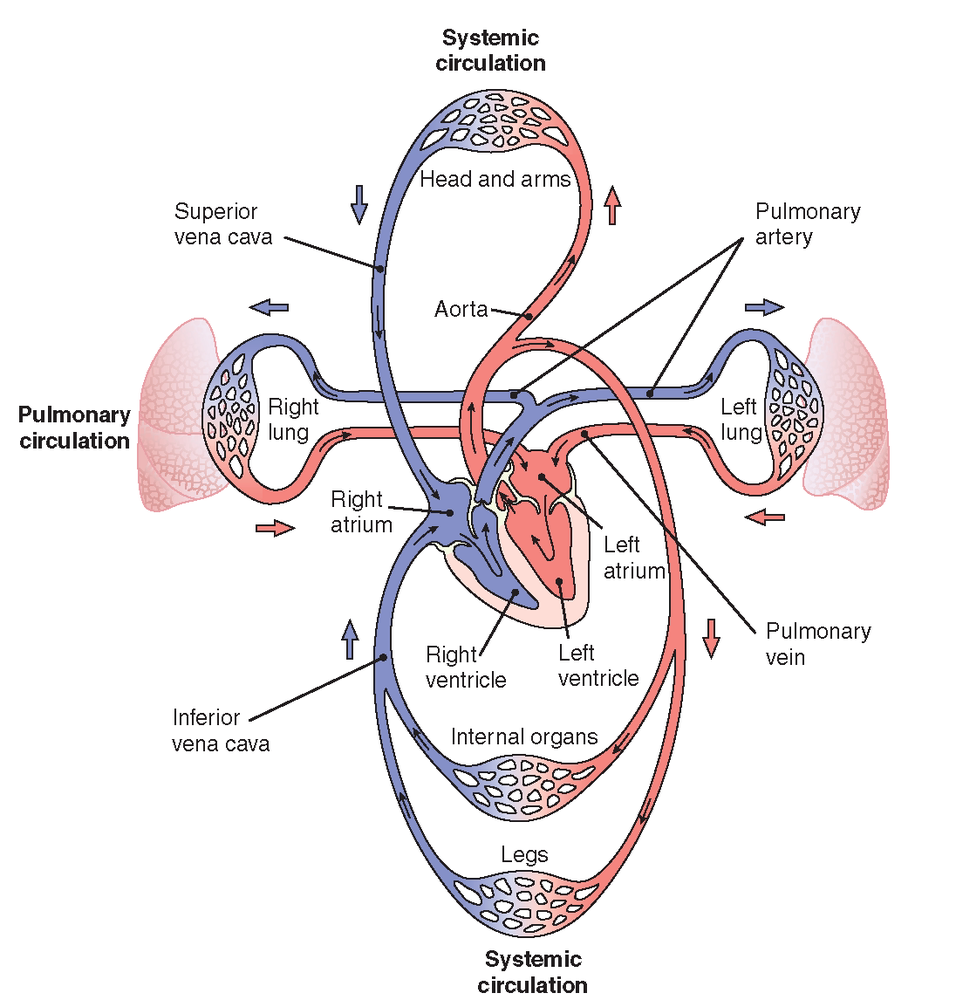
\includegraphics[width=0.7\linewidth]{ImageFiles/Fotopletismografia/SistemaCircolatorio}
	\caption{Rappresentazione del sistema circolatorio.}
	\label{fig:SistemaCircolatorio}
\end{figure}
\begin{itemize}
	\item la \textit{circolazione polmonare}, o piccola circolazione, che include i vasi che dal ventricolo destro del cuore si capillarizzano a livello degli alveoli polmonari e ritornano al cuore nell'atrio sinistro tramite le \textit{vene polmonari};
	\item la \textit{circolazione sistemica}, o grande circolazione, che permette al sangue di scorrere dal ventricolo sinistro all'interno dell'\textit{aorta} per poi raggiungere tutto il corpo e ritornare, grazie alla \textit{vena cava}, all'atrio destro.
\end{itemize}
Tuttavia, la distinzione nei due circuiti è puramente teorica e, in realtà, i due sono strettamente interdipendenti \cite{Cutfield1983}. In effetti, il sangue deossigenato, proveniente dalla circolazione sistemica, ritorna all'atrio destro attraverso la vena cava superiore e inferiore. Durante la fase di \textit{diastole}, scorre nel ventricolo destro attraverso la \textit{valvola tricuspide} e successivamente, grazie alla contrazione del ventricolo (fase di \textit{diastole}), viene spinto nell'arteria polmonare destra e sinistra, che portano il sangue ai polmoni. Grazie ai capillari polmonari avviene il processo di \textit{ematosi}, durante il quale il sangue assimila ossigeno e cede anidride carbonica. Le vene polmonari raccolgono il sangue appena ossigenato e lo conducono nell'atrio sinistro. A questo punto, si ha il confine di passaggio dalla circolazione polmonare alla circolazione sistemica. Dall'atrio destro, attraverso la \textit{valvola bicuspide}, il sangue procede verso il ventricolo sinistro nella la fase di diastole. In seguito, la sistole costringe il sangue nell'aorta che diramandosi fino ai capillari permette la perfusione in tutti i tessuti. Infine, il sangue viene riportato all'atrio destro attraverso le vene cave superiore e inferiore. Il ciclo può ora ripartire. 

\subsection{La circolazione: Pressione, Flusso e Resistenza}
Il sangue è assimilabile a un fluido e, come tale, è in grado di scorrere solamente se è presente un \textit{gradiente di pressione} nei vasi sanguigni. Più precisamente, liquidi e gas fluisco da regioni a maggiore pressione verso regioni a minore pressione. Negli esseri umani, il gradiente è mantenuto grazie alle contrazioni del cuore. Infatti, il sangue esce dal cuore con una pressione elevata e fluisce nei circuiti chiusi dei vasi sanguigni dove la pressione diminuisce progressivamente.\cite{SilverthornDeeUnglaub2020Fu:u}.
Come mostrato nella figura \Fig~\ref{fig:PressioneSangue}, all'interno dell'aorta la pressione è mediamente alta e pari a circa 100 mm Hg. Più precisamente, la pressione risulta essere pulsante con dei picchi di 120 mm Hg (\textit{pressione sistolica}) e dei minimi di 80 mm Hg (\textit{pressione diastolica}).
\begin{figure}[h]
 	\centering
 	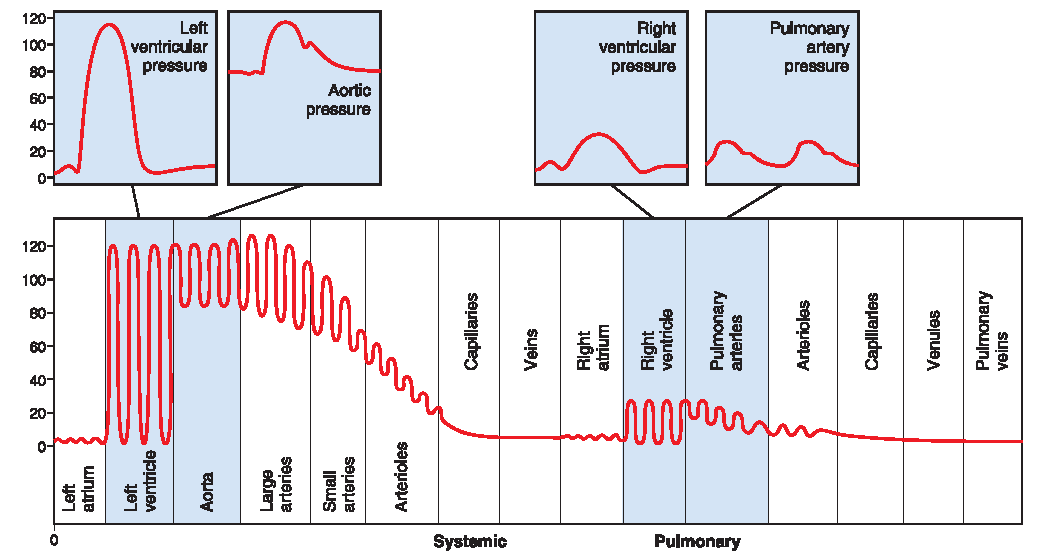
\includegraphics[width=0.9\linewidth]{ImageFiles/Fotopletismografia/PressioneSangue}
 	\caption{Pressione del sangue nelle differenti porzioni dell'apparato circolatorio quando una persona è in posizione supina.}
 	\label{fig:PressioneSangue}
\end{figure}
Mentre il sangue scorre all'interno della circolazione sistemica, la pressione media scende progressivamente fino a circa 0 mm Hg, alla terminazione della vena cava superiore e inferiore. Inoltre, anche l'andamento pulsatile tende a diminuire a livello capillare e venoso. Si noti come, nella circolazione polmonare, la pressione nelle arterie polmonari ritorni ad essere pulsatile, a causa dell'azione del ventricolo destro, ma con una pressione media di 16 mm Hg, di molto inferiore rispetto a quella dell'aorta. La bassa pressione all'interno della piccola circolazione è necessaria per permettere lo scambio gassoso a livello polmonare.

La diminuzione della pressione del flusso ematico all'interno dell'apparato circolatorio è causato dalla \textit{resistenza vascolare}, che rappresenta la frizione tra il liquido e le pareti vascolari. Il flusso attraverso i vasi sanguigni può essere quindi calcolato con la seguente formula, chiamata \textit{legge di Ohm}:
\begin{equation}
	F=\frac{\Delta P}{R}
	\label{eq:OhmsLaw}
\end{equation}
dove \textit{F} è il flusso del sangue, \textit{$\Delta$P} è il gradiente di pressione tra le due estremità di un vaso e \textit{R} è la resistenza  (\Fig~\ref{fig:FlussoSangue}).
\begin{figure}[h]
	\centering
	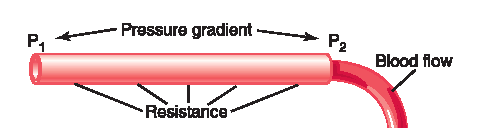
\includegraphics[width=0.7\linewidth]{ImageFiles/Fotopletismografia/FlussoSangue}
	\caption{Relazione tra pressione, resistenza e flusso ematico.P\ped{1}, pressione all'inizio del vaso, P\ped{2}, pressione all'altro capo del vaso}
	\label{fig:FlussoSangue}
\end{figure}
Il flusso indica la quantità di sangue che passa in un dato punto della circolazione in un intervallo di tempo specificato. \`E espresso in millimetri o litri al minuto. Tipicamente in un essere umano adulto il flusso è di circa 5000 ml/min.

Quando il sangue scorre con un ritmo constante all'interno di un vaso lungo e liscio, il suo flusso può essere considerato \textit{laminare}. In questo caso, la velocità del liquido ematico che si trova nel centro del vaso è maggiore rispetto a quello che si trova alle estremità, le cui particelle sono soggette alla forza d'attrito causata dal contatto con le pareti. Questo effetto è chiamato \textit{profilo parabolico della velocità del flusso del sangue} ed è mostrato nella figura \Fig~\ref{fig:FlussoParabolico}.
\begin{figure}[h]
	\centering
	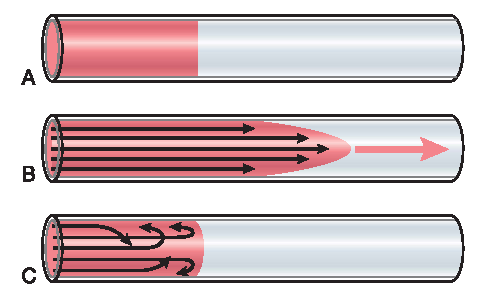
\includegraphics[width=0.7\linewidth]{ImageFiles/Fotopletismografia/FlussoParabolico}
	\caption{\textbf{A}. Due fluidi prima che il flusso inizi.\textbf{B}. Lo stesso fluido un secondo dopo l'inizio del flusso. \textbf{C}. Flusso turbolento}
	\label{fig:FlussoParabolico}
\end{figure}
Quando il ritmo diventa elevato oppure incontra una superficie ruvida o un ostacolo, il flusso non può più essere considerato laminare. Si parla quindi di \textit{flusso turbolento}, caratterizzato da un moto disordinato delle particelle del sangue che causa un aumento della resistenza.

La \textit{pressione idrostatica} del sangue rappresenta la forza esercitata dal sangue su una qualsiasi unità di area della parete di un vaso. In verità, il sangue è un liquido in movimento. Per cui, esso ha una componente dinamica da tenere in considerazione, che rappresenta l'energia cinetica del sistema. In particolare, come si è già visto analizzando il gradiente di pressione nell'apparato cardiocircolatorio, la pressione di un liquido in movimento diminuisce con la distanza percorsa, a causa dell'energia dispersa dall'attrito con le pareti del contenitore. La pressione all'interno dell'apparato circolatorio viene comunemente definita idrostatica, sebbene il sangue sia un fluido in movimento. Un'altra grandezza importante dell'emodinamica (branca della fisiologia cardiovascolare che studia il comportamento del sangue in movimento nei vasi) è la \textit{conduttanza}, che rappresenta l'attitudine di un vaso ad essere percorso dal sangue, fissato un gradiente di pressione. \`E evidente che la conduttanza è il reciproco della resistenza: 
\begin{equation}
	Conduttanza=\frac{1}{Resistenza}
	\label{eq:Conduttanza}
\end{equation}
Inoltre, la conduttanza è strettamente legata al diametro del vaso: 
\begin{equation}
	Conduttanza\propto Diametro^4
	\label{eq:ConduttanzaeDiametro}
\end{equation}
La conduttanza diminuisce al diminuire del diametro perché tutto il sangue può essere considerato a contatto con le pareti e soggetto alla resistenza. Al contrario, se il raggio aumenta, solo le particelle più esterne saranno soggette alla frizione, determinando una velocità maggiore delle particelle nel centro del vaso.
Integrando le diverse velocità delle particelle del sangue lungo una sezione di un vaso sanguigno, si può ricavare la seguente formula (\textit{legge di Poiseuille}):
\begin{equation}
	F\xrightarrow{}\frac{\pi\Delta P r^4}{8 \eta l}
	\label{eq:PoiseuuilleLaw}
\end{equation}
dove \textit{F} è la velocità del sangue, \textit{$\Delta$P} è il gradiente di pressione, \textit{r} è il raggio del vaso, \textit{l} la lunghezza del vaso e \textit{$\eta$} è la viscosità del sangue. Si ponga ancora l'attenzione sulla dipendenza della velocità del flusso con la quarta potenza del raggio del vaso. Quindi, il controllo del flusso del sangue può essere effettuato controllando il diametro dei vasi sanguigni. Questo permette alle arteriole di variare il flusso sanguigno nei tessuti. Al contrario, la lunghezza e la viscosità del sangue (che dipende dal rapporto tra eritrociti e plasma) possono essere considerati parametri costanti che non influenzano la pressione in modo significativo.

\section{Principio di funzionamento}
La fotopletismografia (PPG) è una tecnica ottica, semplice ed economica, che permette di rilevare variazioni del volume del sangue nel letto microvascolare dei tessuti\cite{Dey2019}. Una sorgente luminosa, tipicamente uno o più LED, proietta delle onde luminose sulla pelle, che vengono trasmesse, o riflesse, e acquisite da un fotorilevatore, spesso costituito da un fotodiodo. Poiché il volume del sangue cambia con il ciclo cardiaco, anche l'intensità rilevata subirà delle variazioni. Si tratta di una tecnologia non invasiva spesso utilizzata per misurazioni della frequenza cardiaca e del grado di ossigenazione del sangue (\textit{S\ped{p}O\ped{2}}). Il successo di questa tecnologia è legato alla possibilità di essere inserita all'interno di dispositivi indossabili, come ad esempio smartwatch e pulsossimetri, grazie alle ridotte dimensioni dei moduli. Si stima che la sua diffusione è destinata ad aumentare nel decennio 2020-2030. Pur essendo una tecnologia introdotta nel 1937, l'interesse da parte dei ricercatori è fortemente cresciuto nell'ultimo decennio, come mostra la figura \Fig~\ref{fig:TrendStudies}.   
\begin{figure}[h]
	\centering
	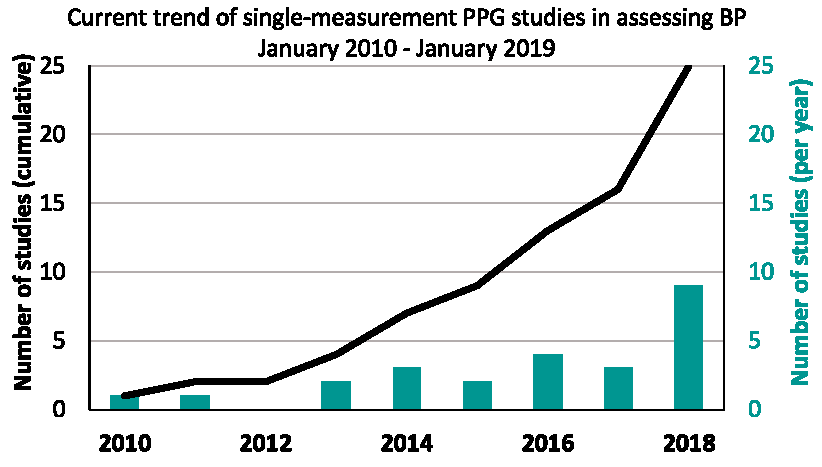
\includegraphics[width=0.7\linewidth]{ImageFiles/Fotopletismografia/TrendStudies}
	\caption{Andamento complessivo delle pubblicazioni che hanno utilizzato la tecnologia PPG a singola misura per stimare la PA da gennaio 2010 a gennaio 2019}
	\label{fig:TrendStudies}
\end{figure}
Originariamente, l'analisi del segnale PPG era utilizzato per il monitoraggio continuo della frequenza cardiaca di pazienti in ospedale, utilizzando dei dispositivi che venivano indossati sulle dita della mano. Un'altra importante applicazione della fotopletismografia è il monitoraggio dell'ossigenazione del sangue di pazienti affetti da COVID-19. Infatti, si è notato come, negli stadi più gravi della malattia, uno dei parametri da tenere in considerazione per valutare le condizioni dei pazienti è l'ossigenazione del sangue. La facilità dell'utilizzo di questi dispositivi ne ha permesso il monitoraggio a domicilio. In condizioni di salute ottimali, l'ossigenazione del sangue si attesta intorno a valori dal 97\% al 99\%. Per questo motivo, se un paziente presenta un livello basso, tipicamente inferiore al 90\%, necessita immediatamente dell'attenzione di un medico. Inoltre, sono stati redatti diversi studi che indicano che l'analisi congiunta dell'onda PPG e dei tracciati ECG sembra essere utile nel diagnosticare e monitorare diverse patologie cardiovascolari, come ad esempio l'ipertensione\cite{Elgendi2019}. 

Esistono due differenti configurazioni per effettuare misurazioni fotopletismografiche (\Fig~\ref{fig:FlussoParabolico}). 
\begin{figure}[h]
	\centering
	\includegraphics[width=0.7\linewidth]{ImageFiles/Fotopletismografia/PPGTrasmissivaRiflettiva}
	\caption{a)PPG modalità riflessiva. b)PPG modalità trasmissiva}
	\label{fig:PPGTrasmissivaRiflettiva}
\end{figure}
La modalità \textit{riflessiva}, in cui la sorgente luminosa e il fotorivelatore sono posti sullo stesso piano. In questo modo, il fotorivelatore rileverà la luce che viene riflessa dal tessuto. Al contrario, nella modalità \textit{trasmissiva}, il fotorilevatore è posto dal lato opposto del tessuto rispetto alla sorgente luminosa. In questo modo, la luce attraversa interamente il tessuto prima di essere acquisita. In genere, viene preferita la modalità riflessiva. Infatti, sebbene la configurazione trasmissiva permetta di ottenere segnali migliori, la modalità a riflessione consente di costruire sensori più comodi e piccoli, mantenendo una buona qualità dei segnali.

La fotopletismografia è considerata una delle tecniche migliori per acquisizioni non invasive basate sul rilevamento degli impulsi periferici\cite{Nenova2009}. Come si è già evidenziato, i principali vantaggi di questa tecnologia sono legati alla sua relativa semplicità di utilizzo e basso costo di realizzazione, garantendo però un'elevata sensitività nella rilevazione nelle variazioni del flusso sanguigno nei tessuti. Inoltre, soprattutto nella configurazione riflessiva, le misurazioni possono essere effettuate in diverse parti del corpo e il suo posizionamento non risulta essere particolarmente critico. Tuttavia, bisogna analizzare alcune criticità che devono essere considerate per ottenere segnali PPG affidabili. La qualità dell'onda PPG è molto sensibile agli artefatti introdotti dal movimento dell'individuo durante l'acquisizione. Infatti, si potrebbero ottenere delle distorsioni nel segnale dovute al movimento relativo tra sensore e tessuto. In aggiunta, è bene scegliere siti con un alto indice di perfusione, come i lobi delle orecchie\todo{ti risulta?}, in modo che la misurazione sia più robusta. Anche la temperatura superficiale della pelle (SST) e ambientale è un fattore che può influenzare alcuni parametri cardiovascolari stimati a partire dal segnale PPG\cite{Jeong2014}. Anche la presenza di sorgenti luminose esterne, quali la luce solare o delle lampade a fluorescenza, possono disturbare l'acquisizione, interferendo con la luce riflessa dalla pelle. \`E necessario quindi studiare dei componenti, come ad esempio l'ALC (\textit{Ambient Light Cancellation}) che permettono di compensare l'effetto dovuto a questi disturbi \cite{Kim2015}.\todo{citazione da valutare}Infine, è importante anche isolare il LED e il fotorilevatore, soprattutto nella modalità riflessiva. In questo modo si evita che la luce possa raggiungere il fotodiodo senza aver attraversato i tessuti.

\todo{introdurre confronto con ECG?}
\todo{nell'articolo Blood Pressure Estimation from Photoplethysmogram relazione tra pressione e segnale ppg}
\pagebreak